\documentclass[12pt, fleqn, paper=letter, oneside]{scrartcl}

\newcommand{\includehead}{true}
\newcommand{\includefoot}{true}

% set basic page format
\usepackage[headsepline=\includehead, footsepline=\includefoot]{scrlayer-scrpage} 
\usepackage[margin=0.5in,
%    footskip=1.5\baselineskip, headsep=0.5\baselineskip,
    includehead=\includehead, includefoot=\includefoot]{geometry}   %Fixed margins
\usepackage[compact]{titlesec}

%\usepackage{setspace}
%\onehalfspace
%\doublespace    

% image support
\renewcommand{\topfraction}{0.85}   %Fixes float spacing
\renewcommand{\textfraction}{0.1}
\renewcommand{\floatpagefraction}{0.75}
\usepackage{graphicx}
	\graphicspath{{/Users/fred/Library/TeXShop/Images/}{./Images/}}
\usepackage[space]{grffile}		

% symbol support
\usepackage{siunitx}    %SI unit : \si{\'unit'} or \SI{#}{\'unit'}
\sisetup{detect-all}
\usepackage{chemfig}    %Write chemical formulas
\usepackage{mathtools}  %Basic math an extension of amsmath

% formatting support
\usepackage{multicol}   %Multiple cols body : command \multicols{#}{'text'}
\usepackage{multirow}   %Multiple row spanning in tables : \multirow{#}{width}{'text'}
\usepackage{enumitem}   %Enumeration control
\usepackage{hyperref} % hyperlinks
\usepackage{soul} % highlighting with \hl{command}


% font and date format
\usepackage{newtxtext}
\setkomafont{disposition}{\bfseries}
\usepackage{fancyref}           %Automatically adds Table (tab:' ') or Figure (fig:' ')
\usepackage{texdate}
\initcurrdate
\def\setdateformat{e\ b\ y\ }
\renewcommand{\headfont}{\normalfont}
\renewcommand{\footfont}{\normalfont}

% useful commands
\newcommand{\biu}[1]{\textbf{\emph{\underline{#1}}}}
\newcommand{\centerframe}[1]{ % this command makes a box around the content
    {\centering\fbox{\begin{minipage}{0.975\columnwidth}#1\end{minipage}}}}

% document commands
\ihead{Name:}
\chead{Hour:}
\ifoot{Revised \printdate}
\cfoot{\maintitle}
\ofoot{\thepage}
\newcommand{\maintitle}{Roller Coaster Toll}

%===================================
\begin{document}
\section{Roller Coaster Toll - Energy Perspective}
\begin{figure}[h]
\centering
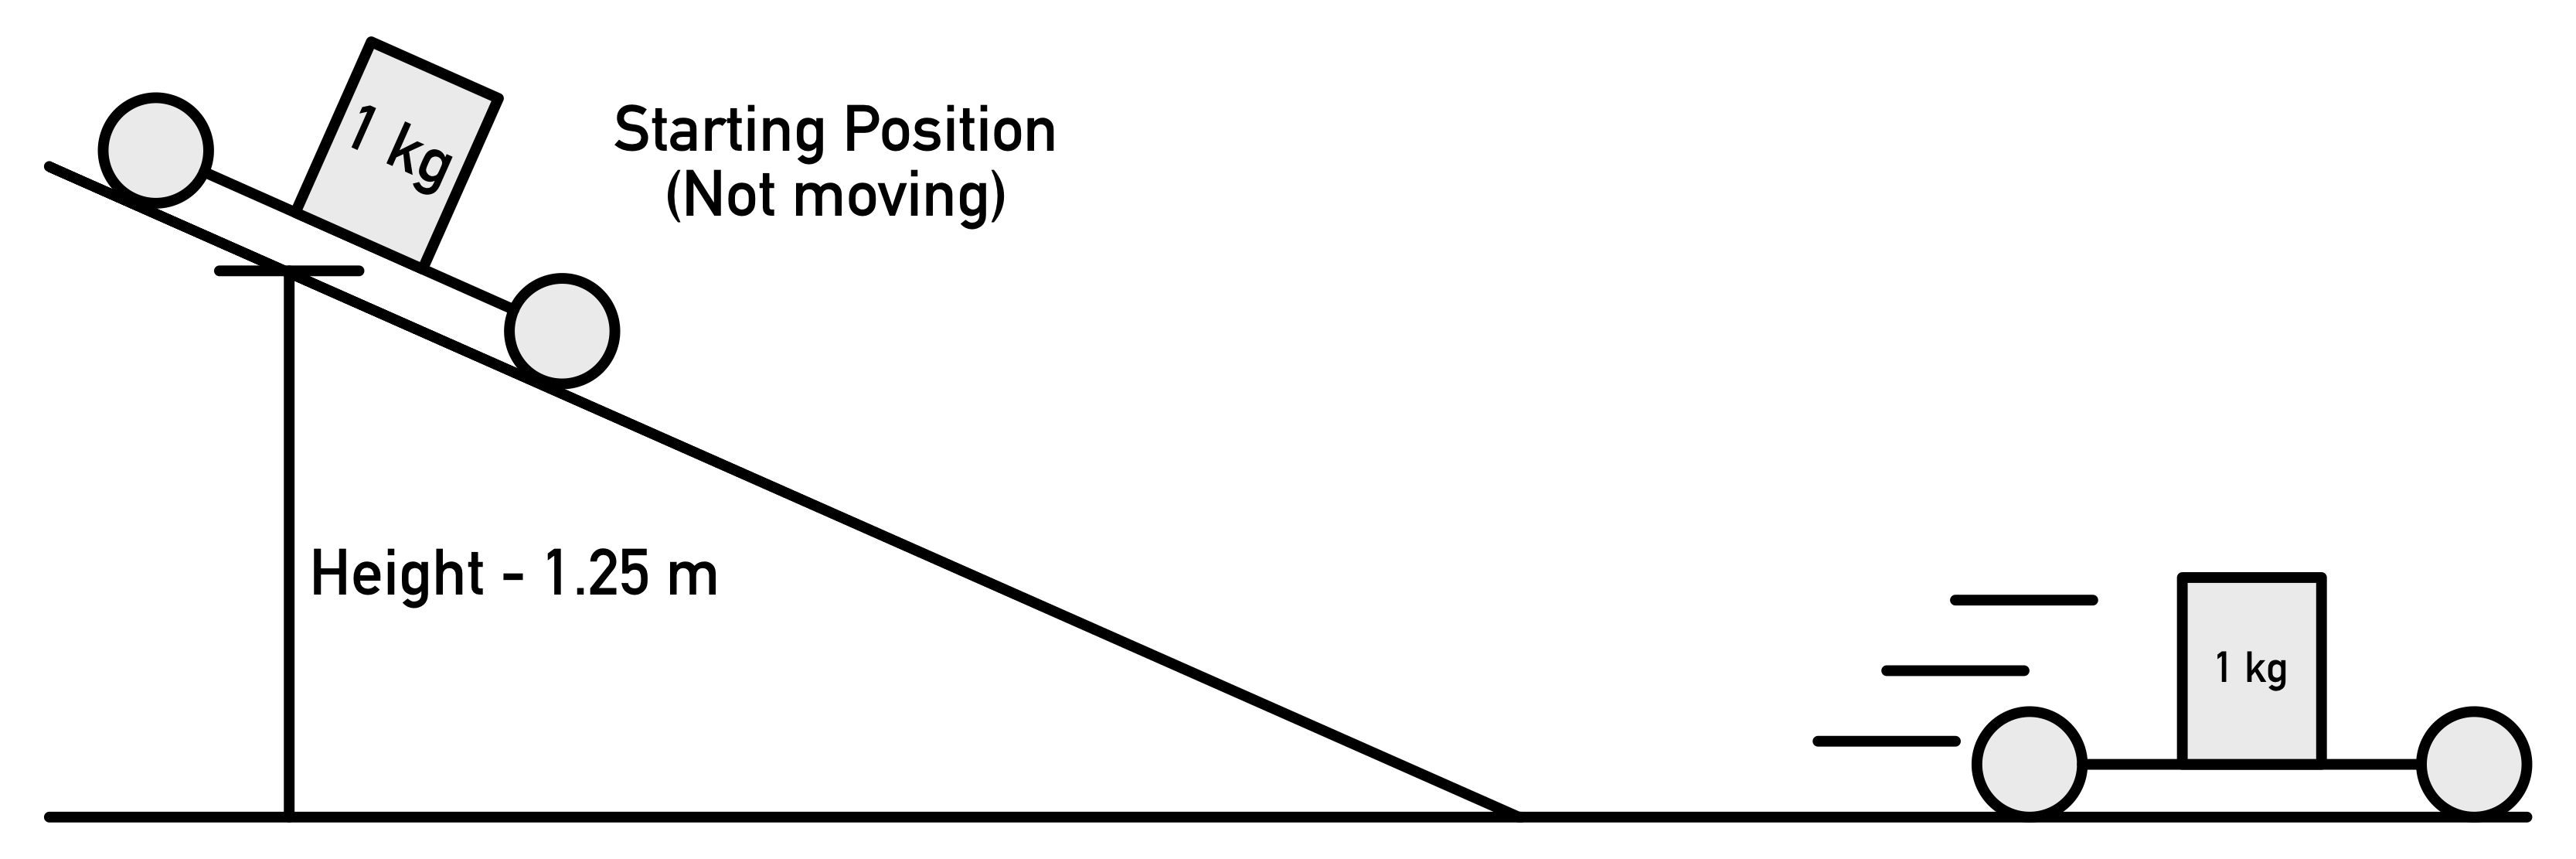
\includegraphics[width=0.6\textwidth]{energycoaster}
\caption{Diagram showing the starting position of a cart on a ramp.  Assume the cart and mass together is 1 kg.}
\end{figure}

\subsection{Potential Energy}
Calculate the potential energy at the starting position.

\emph{To help you work through this worksheet, this one will be done as an example.  When you do the others you should follow almost exactly the same procedure, getting the equation, writing out your reasoning, etc.}

Equation: PE=mgh=(\SI{1}{kg})(\SI{10}{m/s^2})(\SI{1.25}{m})=12.5 J

\subsection{Kinetic Energy}
What is the kinetic energy when the cart is rolling on the flat ground at the bottom of the ramp?
Why is this the kinetic energy, what is your reasoning?

\vfill
\subsection{Final Velocity}
Calculate the final velocity for the cart when it is rolling in the flat part.

\vfill
\subsection{Momentum}
Calculate the momentum of the cart as it is rolling in the flat part.

\vfill
\subsection{Average Force}
Calculate the average force on the cart as it is accelerating down the ramp.  It takes 1.5 s for the cart to travel down the ramp.
\vfill

\clearpage
\section{Roller Coaster Toll - Average Velocity Perspective}
\begin{figure}[h]
\centering
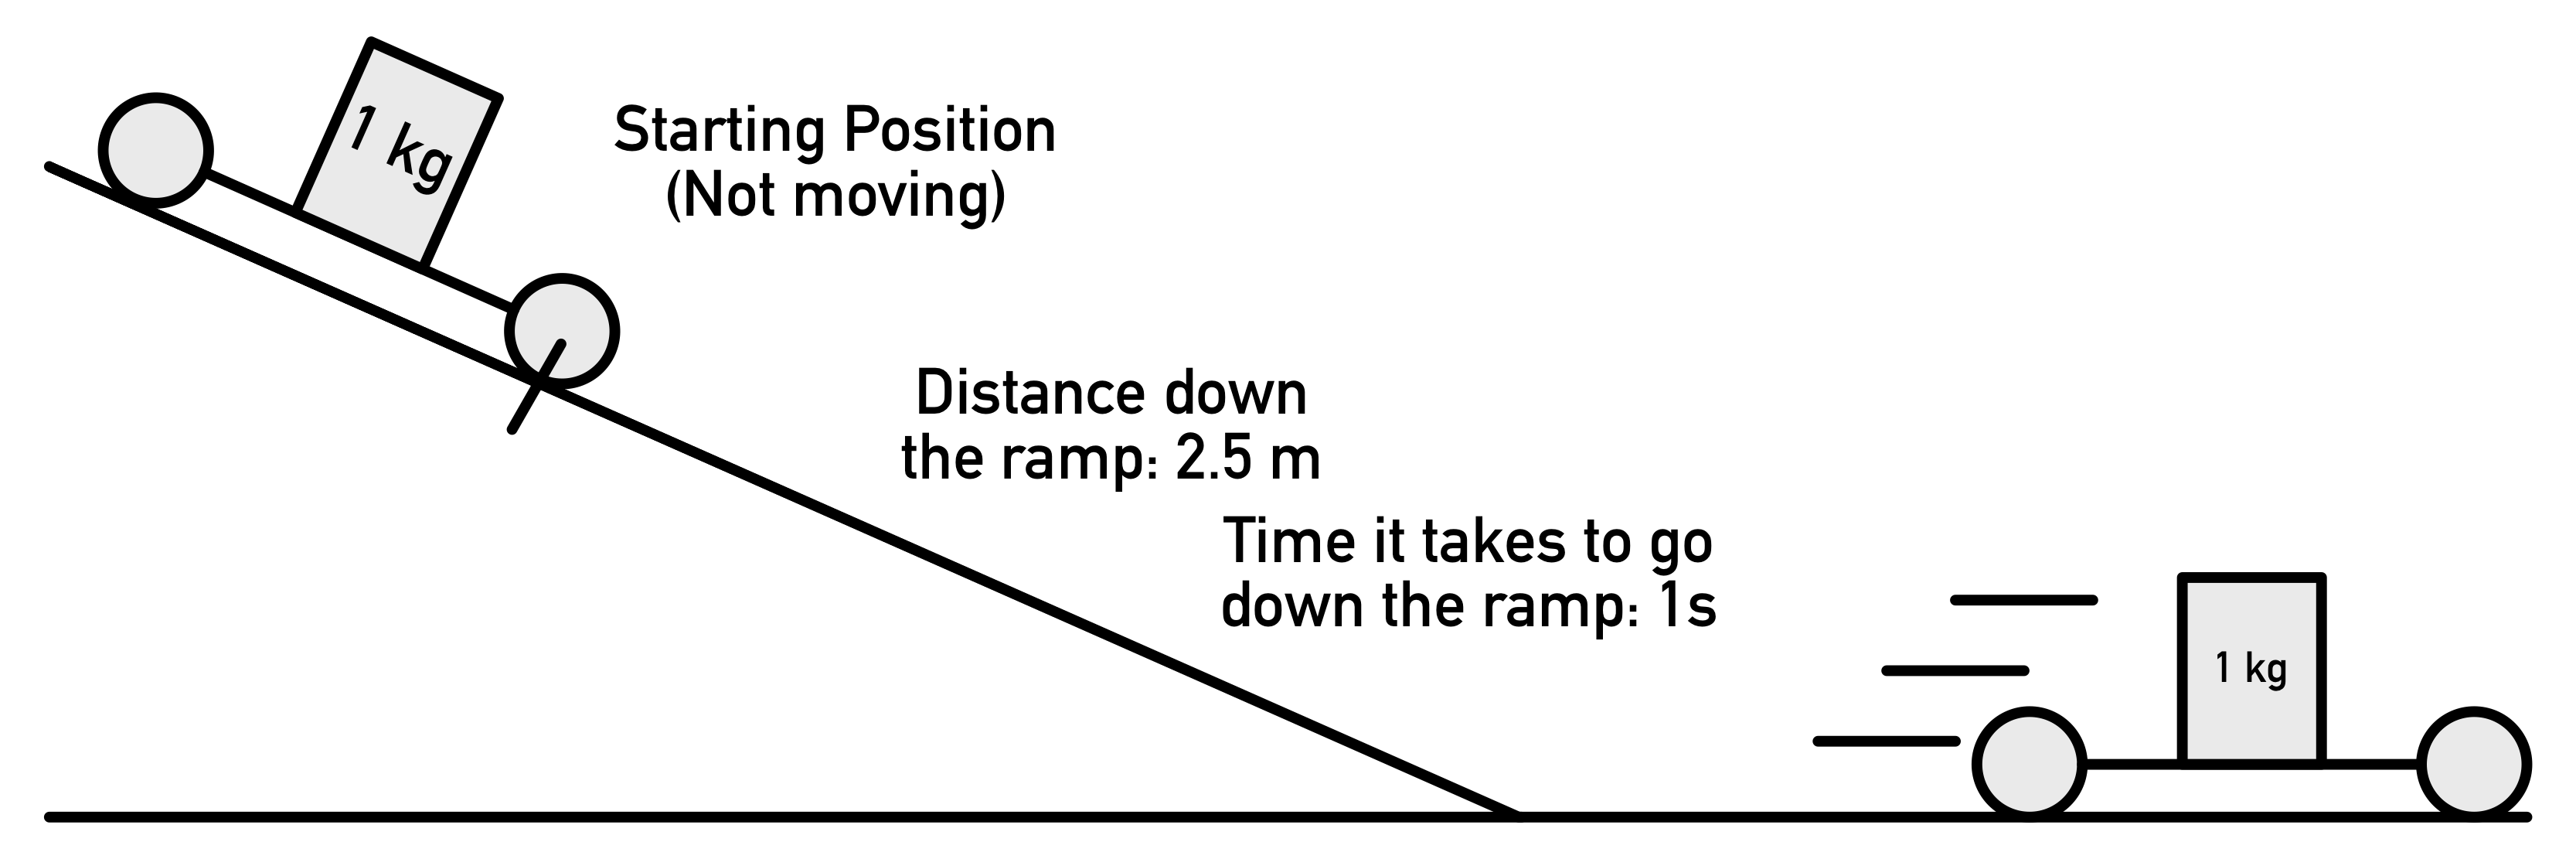
\includegraphics[width=0.6\textwidth]{averagevelocity}
\caption{Diagram showing the starting position of a cart on a ramp.  Assume the cart and mass together is 1 kg.}
\end{figure}

\subsection{Velocity}
Calculate the average velocity of the cart.

\vfill
\subsection{Acceleration}
Calculate the average acceleration of the cart as it goes down the ramp.

\vfill
\subsection{Force}
Calculate the average force on the cart as it goes down the ramp.

\vfill
\subsection{Momentum}
Calculate the momentum (assuming your average velocity after it leaves the ramp).

\vfill
\subsection{Kinetic Energy}
Calculate the kinetic energy for the cart when it is at the bottom of the ramp.

\vfill
\subsection{Reflection}
How well do you think the average velocity represents the motion of the cart?  Explain your answer.

\vfill
















































\end{document}